% Visual

\begin{figure}[h]
	\centering
	\begin{minipage}{.5\textwidth}
		\capstart
		\centering
		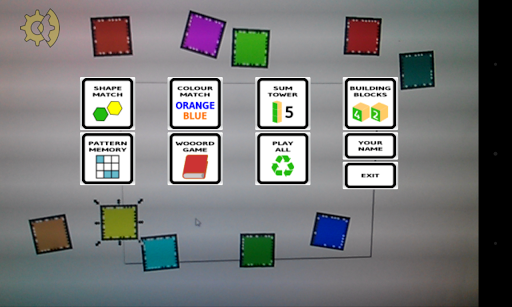
\includegraphics[width=0.9\textwidth]{images/main_menu.png}
		\vspace{-10pt}
		\caption{Screenshot of the main menu.}
		\label{fig:main_menu}
	\end{minipage}%
	\begin{minipage}{.5\textwidth}
		\capstart
		\centering
		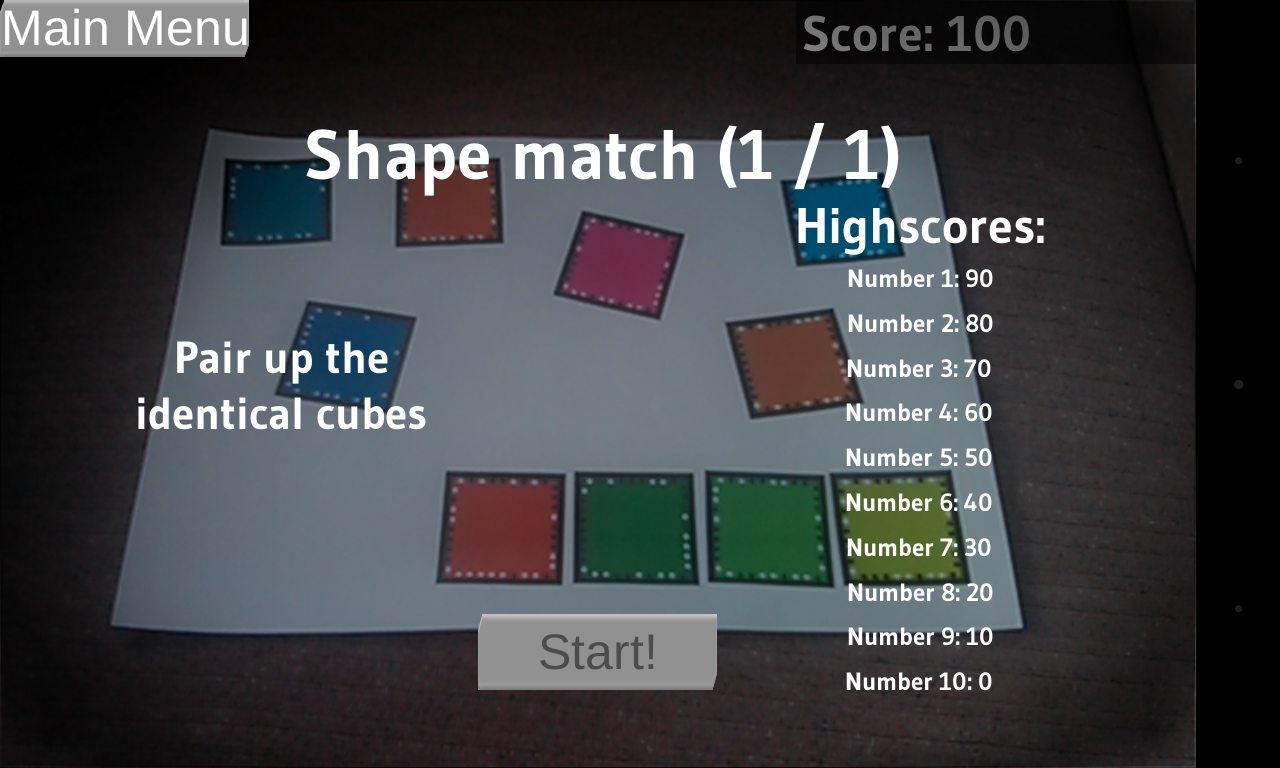
\includegraphics[width=0.9\textwidth]{images/loading_screen.png}
		\vspace{-10pt}
		\caption[Screenshot of a loading screen.]{Loadingscreen for a game.}
		\label{fig:loading_screen}
	\end{minipage}%
\end{figure}

\paragraph{}
The main menu consists of buttons that leads to each minigame with each button having both the name of the corresponding
minigame and a small illustration that gives the user a hint to what the user will do.
There is also the "YOUR NAME" and "EXIT" buttons. The "YOUR NAME" button will take the user to a new screen with a input field 
for changing or setting their username. The "EXIT" button will exit the application.
The camera is always running and we can see the input being rendered to the background.

\paragraph{}
The second picture, \autoref{fig:loading_screen}, shows one of our loading screens, in this case it is the loading screen for \nameref{game:shape_match}.
The loading screens are comprised of two main elements and three smaller elements.
The main elements are the highscore list to the right and a description on the left.
These will introduce the user to what the goal for the minigame is and hopefully encourge the user to do their best everytime to improve the highscore.

The smaller elements are as follows. A titlebar showing game title, current level and how many levels there are in total in that game.
A button in the top left corner that lets the user return to the main menu. Lastly there's the "Start!" button that begins the game.

\begin{figure}[h]
	\centering
	\begin{minipage}{0.48\textwidth}
		\capstart
		\centering
		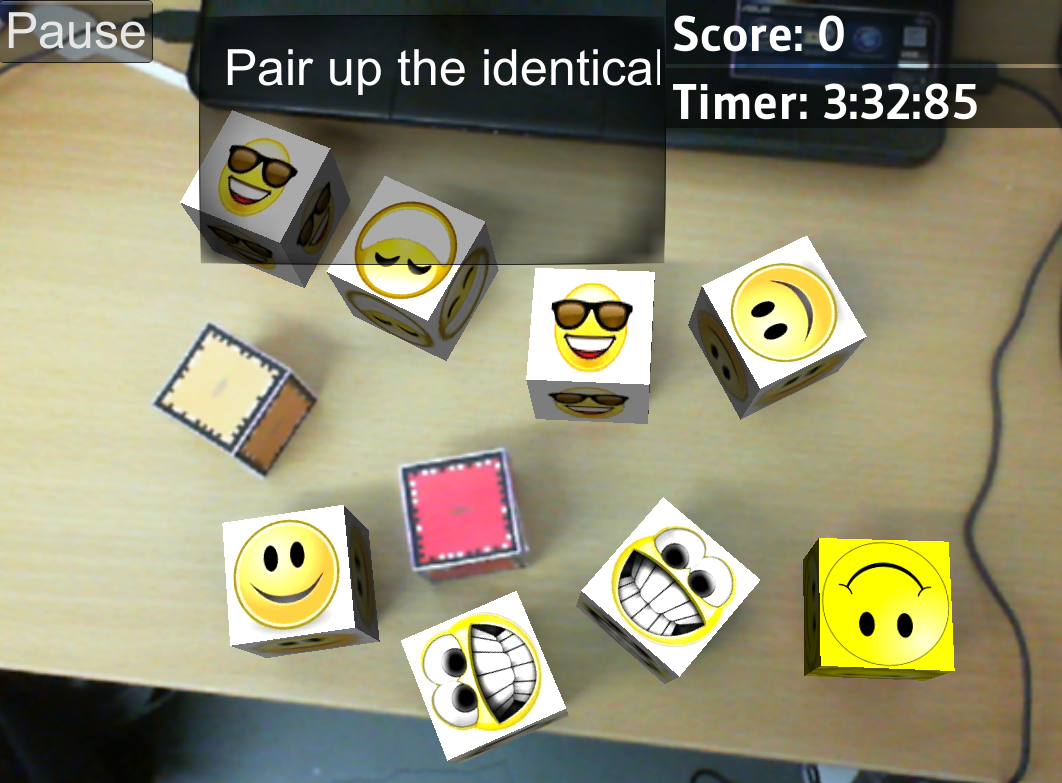
\includegraphics[height=110pt]{images/match_cubes_old}
		\caption[Previous UI in game.]{Early user interface.}
		\label{fig:early_user_interface}
	\end{minipage}
	\begin{minipage}{0.48\textwidth}
		\capstart
		\centering
		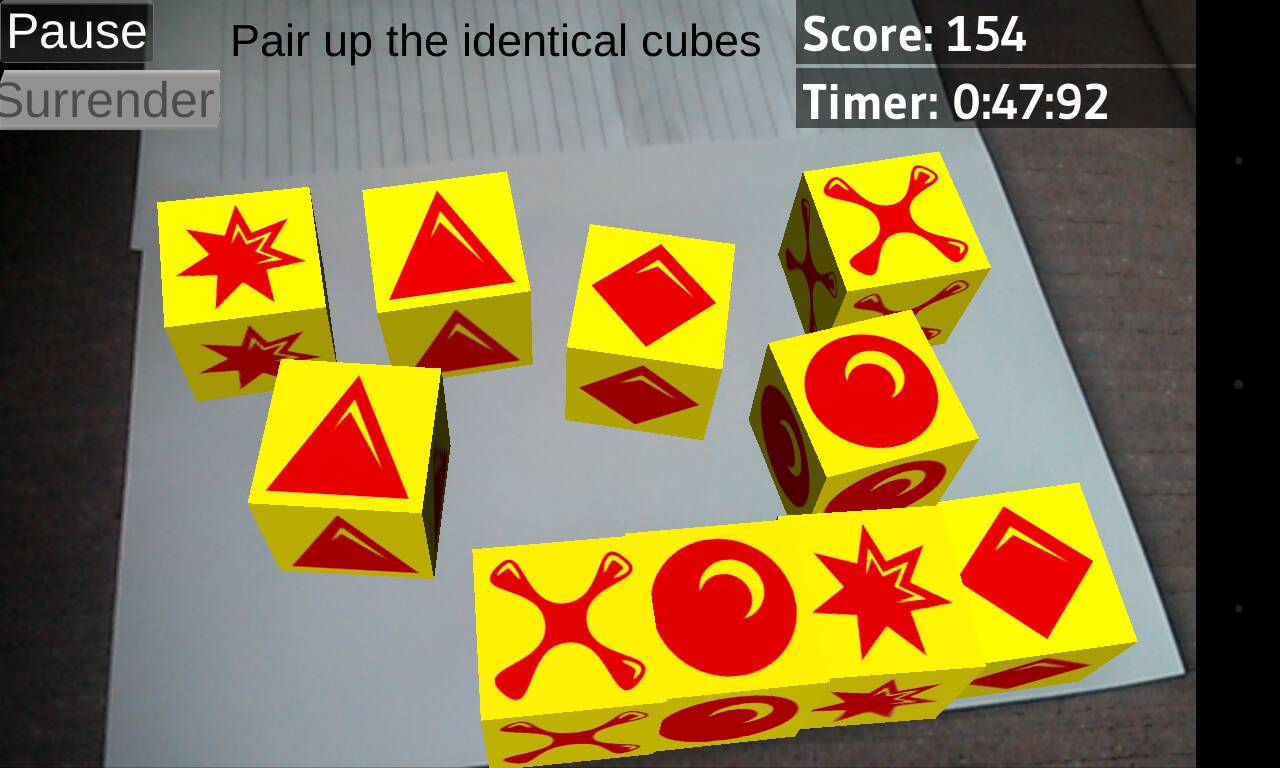
\includegraphics[height=110pt]{images/match_cubes_new}
		\caption[Current UI in game.]{Current user interface.}
		\label{fig:current_user_interface}
	\end{minipage}
\end{figure}

\paragraph{}
\autoref{fig:early_user_interface} and \autoref{fig:current_user_interface} shows our current UI and what we had in the beginning.
Our first version used the default Unity style for both buttons and info boxes.
While it is funcitonal it is not very nice to look at and is too distracting in a enviroment such as this.
To rectify this we created our own UI styles to use instead of the default.
By removing as many distracting elements from the UI as possible we leave much more space open so the user can use more of the
screen to look for the cubes without having the UI getting in the way.



\section{Program flow chart}

\begin{figure}[h]
	\capstart
	\centering
	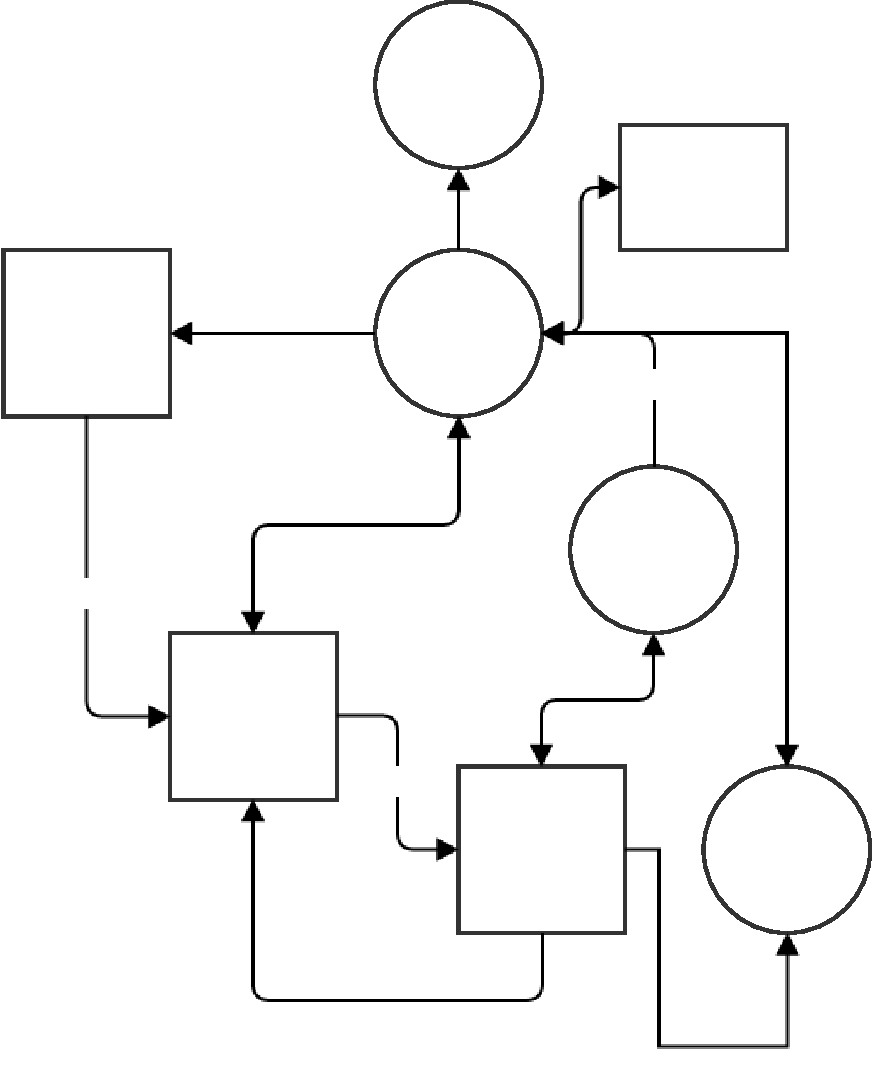
\includegraphics[width=0.8\textwidth]{images/user_flow_chart}
	\caption[Program flow chart]{How a user maneuvers in the program.}
	\label{fig:program_flow_chart}
\end{figure}

Upon starting the program the user is presented with the main menu.
The main menu consists of four different types of buttons.

The first buttons are those that lead to a single mini-game.
When clicked, the player will be taken to the loading screen of the appropriate mini-game. There, the player can read instructions for the game and see current high-scores for that game.
After clicking the play button, the user can start to play the game and the time that effect score will run. While playing, the user can always press pause to get a break.
If the user presses the pause button a pause screen is shown with the options of resuming the game, restarting from level one or go back to the main menu.

When completing a level, the user is taken back to the loading screen if there are more levels left. Otherwise score and position in the high-score list are shown.
From that point the user can only go back to the main menu.

The second type of button are one that is named "Play all games". When the user presses this button it will play all the available mini-games in sequential order.

The next button type are one that changes user. It is called "Change username". When pressing this the user will be presented with a input field where a name can be entered.
This will change the username that is shown in the high-score list. The same name are also used in the logging that are sent to a server.

The last button type will end the program. We only need one of this and it is simply called "Quit".